\documentclass{article} % For LaTeX2e
\usepackage{iclr2019_conference,times}

% Optional math commands from https://github.com/goodfeli/dlbook_notation.
%%%%% NEW MATH DEFINITIONS %%%%%

\usepackage{amsmath,amsfonts,bm}

% Mark sections of captions for referring to divisions of figures
\newcommand{\figleft}{{\em (Left)}}
\newcommand{\figcenter}{{\em (Center)}}
\newcommand{\figright}{{\em (Right)}}
\newcommand{\figtop}{{\em (Top)}}
\newcommand{\figbottom}{{\em (Bottom)}}
\newcommand{\captiona}{{\em (a)}}
\newcommand{\captionb}{{\em (b)}}
\newcommand{\captionc}{{\em (c)}}
\newcommand{\captiond}{{\em (d)}}

% Highlight a newly defined term
\newcommand{\newterm}[1]{{\bf #1}}


% Figure reference, lower-case.
\def\figref#1{figure~\ref{#1}}
% Figure reference, capital. For start of sentence
\def\Figref#1{Figure~\ref{#1}}
\def\twofigref#1#2{figures \ref{#1} and \ref{#2}}
\def\quadfigref#1#2#3#4{figures \ref{#1}, \ref{#2}, \ref{#3} and \ref{#4}}
% Section reference, lower-case.
\def\secref#1{section~\ref{#1}}
% Section reference, capital.
\def\Secref#1{Section~\ref{#1}}
% Reference to two sections.
\def\twosecrefs#1#2{sections \ref{#1} and \ref{#2}}
% Reference to three sections.
\def\secrefs#1#2#3{sections \ref{#1}, \ref{#2} and \ref{#3}}
% Reference to an equation, lower-case.
\def\eqref#1{equation~\ref{#1}}
% Reference to an equation, upper case
\def\Eqref#1{Equation~\ref{#1}}
% A raw reference to an equation---avoid using if possible
\def\plaineqref#1{\ref{#1}}
% Reference to a chapter, lower-case.
\def\chapref#1{chapter~\ref{#1}}
% Reference to an equation, upper case.
\def\Chapref#1{Chapter~\ref{#1}}
% Reference to a range of chapters
\def\rangechapref#1#2{chapters\ref{#1}--\ref{#2}}
% Reference to an algorithm, lower-case.
\def\algref#1{algorithm~\ref{#1}}
% Reference to an algorithm, upper case.
\def\Algref#1{Algorithm~\ref{#1}}
\def\twoalgref#1#2{algorithms \ref{#1} and \ref{#2}}
\def\Twoalgref#1#2{Algorithms \ref{#1} and \ref{#2}}
% Reference to a part, lower case
\def\partref#1{part~\ref{#1}}
% Reference to a part, upper case
\def\Partref#1{Part~\ref{#1}}
\def\twopartref#1#2{parts \ref{#1} and \ref{#2}}

\def\ceil#1{\lceil #1 \rceil}
\def\floor#1{\lfloor #1 \rfloor}
\def\1{\bm{1}}
\newcommand{\train}{\mathcal{D}}
\newcommand{\valid}{\mathcal{D_{\mathrm{valid}}}}
\newcommand{\test}{\mathcal{D_{\mathrm{test}}}}

\def\eps{{\epsilon}}


% Random variables
\def\reta{{\textnormal{$\eta$}}}
\def\ra{{\textnormal{a}}}
\def\rb{{\textnormal{b}}}
\def\rc{{\textnormal{c}}}
\def\rd{{\textnormal{d}}}
\def\re{{\textnormal{e}}}
\def\rf{{\textnormal{f}}}
\def\rg{{\textnormal{g}}}
\def\rh{{\textnormal{h}}}
\def\ri{{\textnormal{i}}}
\def\rj{{\textnormal{j}}}
\def\rk{{\textnormal{k}}}
\def\rl{{\textnormal{l}}}
% rm is already a command, just don't name any random variables m
\def\rn{{\textnormal{n}}}
\def\ro{{\textnormal{o}}}
\def\rp{{\textnormal{p}}}
\def\rq{{\textnormal{q}}}
\def\rr{{\textnormal{r}}}
\def\rs{{\textnormal{s}}}
\def\rt{{\textnormal{t}}}
\def\ru{{\textnormal{u}}}
\def\rv{{\textnormal{v}}}
\def\rw{{\textnormal{w}}}
\def\rx{{\textnormal{x}}}
\def\ry{{\textnormal{y}}}
\def\rz{{\textnormal{z}}}

% Random vectors
\def\rvepsilon{{\mathbf{\epsilon}}}
\def\rvtheta{{\mathbf{\theta}}}
\def\rva{{\mathbf{a}}}
\def\rvb{{\mathbf{b}}}
\def\rvc{{\mathbf{c}}}
\def\rvd{{\mathbf{d}}}
\def\rve{{\mathbf{e}}}
\def\rvf{{\mathbf{f}}}
\def\rvg{{\mathbf{g}}}
\def\rvh{{\mathbf{h}}}
\def\rvu{{\mathbf{i}}}
\def\rvj{{\mathbf{j}}}
\def\rvk{{\mathbf{k}}}
\def\rvl{{\mathbf{l}}}
\def\rvm{{\mathbf{m}}}
\def\rvn{{\mathbf{n}}}
\def\rvo{{\mathbf{o}}}
\def\rvp{{\mathbf{p}}}
\def\rvq{{\mathbf{q}}}
\def\rvr{{\mathbf{r}}}
\def\rvs{{\mathbf{s}}}
\def\rvt{{\mathbf{t}}}
\def\rvu{{\mathbf{u}}}
\def\rvv{{\mathbf{v}}}
\def\rvw{{\mathbf{w}}}
\def\rvx{{\mathbf{x}}}
\def\rvy{{\mathbf{y}}}
\def\rvz{{\mathbf{z}}}

% Elements of random vectors
\def\erva{{\textnormal{a}}}
\def\ervb{{\textnormal{b}}}
\def\ervc{{\textnormal{c}}}
\def\ervd{{\textnormal{d}}}
\def\erve{{\textnormal{e}}}
\def\ervf{{\textnormal{f}}}
\def\ervg{{\textnormal{g}}}
\def\ervh{{\textnormal{h}}}
\def\ervi{{\textnormal{i}}}
\def\ervj{{\textnormal{j}}}
\def\ervk{{\textnormal{k}}}
\def\ervl{{\textnormal{l}}}
\def\ervm{{\textnormal{m}}}
\def\ervn{{\textnormal{n}}}
\def\ervo{{\textnormal{o}}}
\def\ervp{{\textnormal{p}}}
\def\ervq{{\textnormal{q}}}
\def\ervr{{\textnormal{r}}}
\def\ervs{{\textnormal{s}}}
\def\ervt{{\textnormal{t}}}
\def\ervu{{\textnormal{u}}}
\def\ervv{{\textnormal{v}}}
\def\ervw{{\textnormal{w}}}
\def\ervx{{\textnormal{x}}}
\def\ervy{{\textnormal{y}}}
\def\ervz{{\textnormal{z}}}

% Random matrices
\def\rmA{{\mathbf{A}}}
\def\rmB{{\mathbf{B}}}
\def\rmC{{\mathbf{C}}}
\def\rmD{{\mathbf{D}}}
\def\rmE{{\mathbf{E}}}
\def\rmF{{\mathbf{F}}}
\def\rmG{{\mathbf{G}}}
\def\rmH{{\mathbf{H}}}
\def\rmI{{\mathbf{I}}}
\def\rmJ{{\mathbf{J}}}
\def\rmK{{\mathbf{K}}}
\def\rmL{{\mathbf{L}}}
\def\rmM{{\mathbf{M}}}
\def\rmN{{\mathbf{N}}}
\def\rmO{{\mathbf{O}}}
\def\rmP{{\mathbf{P}}}
\def\rmQ{{\mathbf{Q}}}
\def\rmR{{\mathbf{R}}}
\def\rmS{{\mathbf{S}}}
\def\rmT{{\mathbf{T}}}
\def\rmU{{\mathbf{U}}}
\def\rmV{{\mathbf{V}}}
\def\rmW{{\mathbf{W}}}
\def\rmX{{\mathbf{X}}}
\def\rmY{{\mathbf{Y}}}
\def\rmZ{{\mathbf{Z}}}

% Elements of random matrices
\def\ermA{{\textnormal{A}}}
\def\ermB{{\textnormal{B}}}
\def\ermC{{\textnormal{C}}}
\def\ermD{{\textnormal{D}}}
\def\ermE{{\textnormal{E}}}
\def\ermF{{\textnormal{F}}}
\def\ermG{{\textnormal{G}}}
\def\ermH{{\textnormal{H}}}
\def\ermI{{\textnormal{I}}}
\def\ermJ{{\textnormal{J}}}
\def\ermK{{\textnormal{K}}}
\def\ermL{{\textnormal{L}}}
\def\ermM{{\textnormal{M}}}
\def\ermN{{\textnormal{N}}}
\def\ermO{{\textnormal{O}}}
\def\ermP{{\textnormal{P}}}
\def\ermQ{{\textnormal{Q}}}
\def\ermR{{\textnormal{R}}}
\def\ermS{{\textnormal{S}}}
\def\ermT{{\textnormal{T}}}
\def\ermU{{\textnormal{U}}}
\def\ermV{{\textnormal{V}}}
\def\ermW{{\textnormal{W}}}
\def\ermX{{\textnormal{X}}}
\def\ermY{{\textnormal{Y}}}
\def\ermZ{{\textnormal{Z}}}

% Vectors
\def\vzero{{\bm{0}}}
\def\vone{{\bm{1}}}
\def\vmu{{\bm{\mu}}}
\def\vtheta{{\bm{\theta}}}
\def\va{{\bm{a}}}
\def\vb{{\bm{b}}}
\def\vc{{\bm{c}}}
\def\vd{{\bm{d}}}
\def\ve{{\bm{e}}}
\def\vf{{\bm{f}}}
\def\vg{{\bm{g}}}
\def\vh{{\bm{h}}}
\def\vi{{\bm{i}}}
\def\vj{{\bm{j}}}
\def\vk{{\bm{k}}}
\def\vl{{\bm{l}}}
\def\vm{{\bm{m}}}
\def\vn{{\bm{n}}}
\def\vo{{\bm{o}}}
\def\vp{{\bm{p}}}
\def\vq{{\bm{q}}}
\def\vr{{\bm{r}}}
\def\vs{{\bm{s}}}
\def\vt{{\bm{t}}}
\def\vu{{\bm{u}}}
\def\vv{{\bm{v}}}
\def\vw{{\bm{w}}}
\def\vx{{\bm{x}}}
\def\vy{{\bm{y}}}
\def\vz{{\bm{z}}}

% Elements of vectors
\def\evalpha{{\alpha}}
\def\evbeta{{\beta}}
\def\evepsilon{{\epsilon}}
\def\evlambda{{\lambda}}
\def\evomega{{\omega}}
\def\evmu{{\mu}}
\def\evpsi{{\psi}}
\def\evsigma{{\sigma}}
\def\evtheta{{\theta}}
\def\eva{{a}}
\def\evb{{b}}
\def\evc{{c}}
\def\evd{{d}}
\def\eve{{e}}
\def\evf{{f}}
\def\evg{{g}}
\def\evh{{h}}
\def\evi{{i}}
\def\evj{{j}}
\def\evk{{k}}
\def\evl{{l}}
\def\evm{{m}}
\def\evn{{n}}
\def\evo{{o}}
\def\evp{{p}}
\def\evq{{q}}
\def\evr{{r}}
\def\evs{{s}}
\def\evt{{t}}
\def\evu{{u}}
\def\evv{{v}}
\def\evw{{w}}
\def\evx{{x}}
\def\evy{{y}}
\def\evz{{z}}

% Matrix
\def\mA{{\bm{A}}}
\def\mB{{\bm{B}}}
\def\mC{{\bm{C}}}
\def\mD{{\bm{D}}}
\def\mE{{\bm{E}}}
\def\mF{{\bm{F}}}
\def\mG{{\bm{G}}}
\def\mH{{\bm{H}}}
\def\mI{{\bm{I}}}
\def\mJ{{\bm{J}}}
\def\mK{{\bm{K}}}
\def\mL{{\bm{L}}}
\def\mM{{\bm{M}}}
\def\mN{{\bm{N}}}
\def\mO{{\bm{O}}}
\def\mP{{\bm{P}}}
\def\mQ{{\bm{Q}}}
\def\mR{{\bm{R}}}
\def\mS{{\bm{S}}}
\def\mT{{\bm{T}}}
\def\mU{{\bm{U}}}
\def\mV{{\bm{V}}}
\def\mW{{\bm{W}}}
\def\mX{{\bm{X}}}
\def\mY{{\bm{Y}}}
\def\mZ{{\bm{Z}}}
\def\mBeta{{\bm{\beta}}}
\def\mPhi{{\bm{\Phi}}}
\def\mLambda{{\bm{\Lambda}}}
\def\mSigma{{\bm{\Sigma}}}

% Tensor
\DeclareMathAlphabet{\mathsfit}{\encodingdefault}{\sfdefault}{m}{sl}
\SetMathAlphabet{\mathsfit}{bold}{\encodingdefault}{\sfdefault}{bx}{n}
\newcommand{\tens}[1]{\bm{\mathsfit{#1}}}
\def\tA{{\tens{A}}}
\def\tB{{\tens{B}}}
\def\tC{{\tens{C}}}
\def\tD{{\tens{D}}}
\def\tE{{\tens{E}}}
\def\tF{{\tens{F}}}
\def\tG{{\tens{G}}}
\def\tH{{\tens{H}}}
\def\tI{{\tens{I}}}
\def\tJ{{\tens{J}}}
\def\tK{{\tens{K}}}
\def\tL{{\tens{L}}}
\def\tM{{\tens{M}}}
\def\tN{{\tens{N}}}
\def\tO{{\tens{O}}}
\def\tP{{\tens{P}}}
\def\tQ{{\tens{Q}}}
\def\tR{{\tens{R}}}
\def\tS{{\tens{S}}}
\def\tT{{\tens{T}}}
\def\tU{{\tens{U}}}
\def\tV{{\tens{V}}}
\def\tW{{\tens{W}}}
\def\tX{{\tens{X}}}
\def\tY{{\tens{Y}}}
\def\tZ{{\tens{Z}}}


% Graph
\def\gA{{\mathcal{A}}}
\def\gB{{\mathcal{B}}}
\def\gC{{\mathcal{C}}}
\def\gD{{\mathcal{D}}}
\def\gE{{\mathcal{E}}}
\def\gF{{\mathcal{F}}}
\def\gG{{\mathcal{G}}}
\def\gH{{\mathcal{H}}}
\def\gI{{\mathcal{I}}}
\def\gJ{{\mathcal{J}}}
\def\gK{{\mathcal{K}}}
\def\gL{{\mathcal{L}}}
\def\gM{{\mathcal{M}}}
\def\gN{{\mathcal{N}}}
\def\gO{{\mathcal{O}}}
\def\gP{{\mathcal{P}}}
\def\gQ{{\mathcal{Q}}}
\def\gR{{\mathcal{R}}}
\def\gS{{\mathcal{S}}}
\def\gT{{\mathcal{T}}}
\def\gU{{\mathcal{U}}}
\def\gV{{\mathcal{V}}}
\def\gW{{\mathcal{W}}}
\def\gX{{\mathcal{X}}}
\def\gY{{\mathcal{Y}}}
\def\gZ{{\mathcal{Z}}}

% Sets
\def\sA{{\mathbb{A}}}
\def\sB{{\mathbb{B}}}
\def\sC{{\mathbb{C}}}
\def\sD{{\mathbb{D}}}
% Don't use a set called E, because this would be the same as our symbol
% for expectation.
\def\sF{{\mathbb{F}}}
\def\sG{{\mathbb{G}}}
\def\sH{{\mathbb{H}}}
\def\sI{{\mathbb{I}}}
\def\sJ{{\mathbb{J}}}
\def\sK{{\mathbb{K}}}
\def\sL{{\mathbb{L}}}
\def\sM{{\mathbb{M}}}
\def\sN{{\mathbb{N}}}
\def\sO{{\mathbb{O}}}
\def\sP{{\mathbb{P}}}
\def\sQ{{\mathbb{Q}}}
\def\sR{{\mathbb{R}}}
\def\sS{{\mathbb{S}}}
\def\sT{{\mathbb{T}}}
\def\sU{{\mathbb{U}}}
\def\sV{{\mathbb{V}}}
\def\sW{{\mathbb{W}}}
\def\sX{{\mathbb{X}}}
\def\sY{{\mathbb{Y}}}
\def\sZ{{\mathbb{Z}}}

% Entries of a matrix
\def\emLambda{{\Lambda}}
\def\emA{{A}}
\def\emB{{B}}
\def\emC{{C}}
\def\emD{{D}}
\def\emE{{E}}
\def\emF{{F}}
\def\emG{{G}}
\def\emH{{H}}
\def\emI{{I}}
\def\emJ{{J}}
\def\emK{{K}}
\def\emL{{L}}
\def\emM{{M}}
\def\emN{{N}}
\def\emO{{O}}
\def\emP{{P}}
\def\emQ{{Q}}
\def\emR{{R}}
\def\emS{{S}}
\def\emT{{T}}
\def\emU{{U}}
\def\emV{{V}}
\def\emW{{W}}
\def\emX{{X}}
\def\emY{{Y}}
\def\emZ{{Z}}
\def\emSigma{{\Sigma}}

% entries of a tensor
% Same font as tensor, without \bm wrapper
\newcommand{\etens}[1]{\mathsfit{#1}}
\def\etLambda{{\etens{\Lambda}}}
\def\etA{{\etens{A}}}
\def\etB{{\etens{B}}}
\def\etC{{\etens{C}}}
\def\etD{{\etens{D}}}
\def\etE{{\etens{E}}}
\def\etF{{\etens{F}}}
\def\etG{{\etens{G}}}
\def\etH{{\etens{H}}}
\def\etI{{\etens{I}}}
\def\etJ{{\etens{J}}}
\def\etK{{\etens{K}}}
\def\etL{{\etens{L}}}
\def\etM{{\etens{M}}}
\def\etN{{\etens{N}}}
\def\etO{{\etens{O}}}
\def\etP{{\etens{P}}}
\def\etQ{{\etens{Q}}}
\def\etR{{\etens{R}}}
\def\etS{{\etens{S}}}
\def\etT{{\etens{T}}}
\def\etU{{\etens{U}}}
\def\etV{{\etens{V}}}
\def\etW{{\etens{W}}}
\def\etX{{\etens{X}}}
\def\etY{{\etens{Y}}}
\def\etZ{{\etens{Z}}}

% The true underlying data generating distribution
\newcommand{\pdata}{p_{\rm{data}}}
% The empirical distribution defined by the training set
\newcommand{\ptrain}{\hat{p}_{\rm{data}}}
\newcommand{\Ptrain}{\hat{P}_{\rm{data}}}
% The model distribution
\newcommand{\pmodel}{p_{\rm{model}}}
\newcommand{\Pmodel}{P_{\rm{model}}}
\newcommand{\ptildemodel}{\tilde{p}_{\rm{model}}}
% Stochastic autoencoder distributions
\newcommand{\pencode}{p_{\rm{encoder}}}
\newcommand{\pdecode}{p_{\rm{decoder}}}
\newcommand{\precons}{p_{\rm{reconstruct}}}

\newcommand{\laplace}{\mathrm{Laplace}} % Laplace distribution

\newcommand{\E}{\mathbb{E}}
\newcommand{\Ls}{\mathcal{L}}
\newcommand{\R}{\mathbb{R}}
\newcommand{\emp}{\tilde{p}}
\newcommand{\lr}{\alpha}
\newcommand{\reg}{\lambda}
\newcommand{\rect}{\mathrm{rectifier}}
\newcommand{\softmax}{\mathrm{softmax}}
\newcommand{\sigmoid}{\sigma}
\newcommand{\softplus}{\zeta}
\newcommand{\KL}{D_{\mathrm{KL}}}
\newcommand{\Var}{\mathrm{Var}}
\newcommand{\standarderror}{\mathrm{SE}}
\newcommand{\Cov}{\mathrm{Cov}}
% Wolfram Mathworld says $L^2$ is for function spaces and $\ell^2$ is for vectors
% But then they seem to use $L^2$ for vectors throughout the site, and so does
% wikipedia.
\newcommand{\normlzero}{L^0}
\newcommand{\normlone}{L^1}
\newcommand{\normltwo}{L^2}
\newcommand{\normlp}{L^p}
\newcommand{\normmax}{L^\infty}

\newcommand{\parents}{Pa} % See usage in notation.tex. Chosen to match Daphne's book.

\DeclareMathOperator*{\argmax}{arg\,max}
\DeclareMathOperator*{\argmin}{arg\,min}

\DeclareMathOperator{\sign}{sign}
\DeclareMathOperator{\Tr}{Tr}
\let\ab\allowbreak



\usepackage{hyperref}
\usepackage{url}
\usepackage{lipsum}
\usepackage{graphicx}
\usepackage{wrapfig}
\usepackage{float}
\usepackage[tmargin=0.59in, bmargin=0.7in, lmargin=0.92in, rmargin=0.92in]{geometry}

\title{Reproducing A Novel Weakly Supervised Clustering Framework and Evaluating Practical Applicability}

% Authors must not appear in the submitted version. They should be hidden
% as long as the \iclrfinalcopy macro remains commented out below.
% Non-anonymous submissions will be rejected without review.


\author{Sameen Islam, Mohammed Mossuily \& Saivignesh Pandian \\
Department of Electronics and Computer Science\\
University of Southampton \\
Southampton, United Kingdom\\
\texttt{\{si1u19, mtm1g19, ssp1e17\}@soton.ac.uk} }

% \And
% Mohammed Mossuily \\
% Department of ECS\\
% University of Southampton \\
% Southampton, United Kingdom\\
% \texttt{mtm1g19@soton.ac.uk} \\

% \And
% Saivignesh Pandian \\
% Department of ECS\\
% University of Southampton \\
% Southampton, United Kingdom\\
% \texttt{ssp1e17@soton.ac.uk}
% }

% The \author macro works with any number of authors. There are two commands
% used to separate the names and addresses of multiple authors: \And and \AND.
%
% Using \And between authors leaves it to \LaTeX{} to determine where to break
% the lines. Using \AND forces a linebreak at that point. So, if \LaTeX{}
% puts 3 of 4 authors names on the first line, and the last on the second
% line, try using \AND instead of \And before the third author name.

\newcommand{\fix}{\marginpar{FIX}}
\newcommand{\new}{\marginpar{NEW}}

\iclrfinalcopy % Uncomment for camera-ready version, but NOT for submission.
\begin{document}


\maketitle

\begin{abstract}
In this investigation we seek to replicate the results of a previously proposed weakly supervised clustering model that exploits unique class count labels. We independently reconstruct the model presented and reproduce the results on the MNIST dataset, achieving a 98.37\% clustering accuracy. Furthermore, we bridge the gap between the proposed model and a future practical deployment by exploring practical limitations of the model with training and implementation.
\end{abstract}

% \section{Outline}
% \begin{itemize}
%     \item Introduction - Sameen
%     \item Mathematical Background - Mohammed
%     \item Project Scope - Mohammed
%     \item Reproducing the Model - Sameen
%     \begin{itemize}
%         \item Model Architecture - Sameen
%         \item Training the Model - Sameen
%     \end{itemize}
%     \item Applying the Model to MNIST - Sai
%     \begin{itemize}
%         \item Autoencoder Model - Sai
%         \item KDE Model - Sai
%         \item Reproduced Results - Sai
%         \item Comparison with Other Models - Sai 
%     \end{itemize}
%     \item Efficacy of Project - Sameen
%     \item Conclusions - Mohammed
% \end{itemize}

\section{Introduction} %[MM]
% The paper we replicate aims to perform semantic segmentation on histological lymph node sections to identify breast cancer in a weakly supervised manner.  The problem this paper tackles provides a path to developing a system where clinicians can readily identify cancerous regions from images of histological lymph node sections without requiring specialist expertise. It further tries to develop on the state-of-the-art by not requiring these humans to hand label image pixels of histological slides to mark cancerous regions. In this paper, we verify the effectiveness of the model on a baseline dataset and provide a critical discussion of the gains purported by \cite{Oner2019}.

In \cite{Oner2019}, they present a weakly supervised model which is trained to predict the number of unique classes in a dataset. They argue that a model trained to do so must be learning some underlying patterns in the data to inform it of the number of classes. Thus, such a model should after training, be able to be re-purposed to predict the class labels on specific instances of data. This is presented to be of great use in fields such as the medical profession, in which one might know the number of cancerous cells in an image, but not be able to identify which pixels in the image correspond to such a cell. 

% Thus, the paper aims to provide the proof of concept for a path to developing a system where clinicians can readily identify cancerous regions from images of histological lymph node sections without requiring specialist expertise or hand labelled image pixels of histological slides. 

% The problem is framed as a multiple instance learning (MIL) problem where bags of instances and bag level labels are used as input data, whereby the goal of the model is to identify the number of unique classes of instances in the bag. The model can then be used to label instances of data. As such, it is possible to generalise to other domains.

\section{Experimental Methodology}
While the specific code for the model is provided and available\footnote{http://bit.ly/uniqueclasscount}, we found that it was poorly documented and improperly motivated. Thus in this investigation, we completely re-implemented the model \footnote{https://github.com/COMP6248-Reproducability-Challenge/UCC-Classifier}, which allowed us to explore the architecture and understand the motivations behind certain choices. 

We seek to provide some reasoning behind the model choices made in the original paper, as well as bridge the gap in knowledge needed to implement and deploy such a model. For example, as the original paper makes no reference to the training time and difficulty, we seek to analyse whether such a model can be considered practical when the computational costs are also taken into account. Finally, we seek to replicate the results found in the original paper, and compare with other novel techniques to draw conclusions about the efficacy of this presented model.
% \section{Project Scope} %[MM]

For this investigation, we have limited the scope to only reproducing and exploring the presented model on the MNIST dataset. \cite{Oner2019} make no mention as to the training difficulty of their model. However, we found that the training times for useful results were unreasonably long on the MNIST dataset, and training on other datasets such as CIFAR or CAMELYON were considerably slower. As such, only MNIST data is used in this project.

\section{Reproducing the Model} %[SI]
% The original paper experiments on the MNIST, CIFAR10, CIFAR100 and other datasets on breast cancer metastases. In this paper, we limit the scope of our project to the successful reproduction of the results obtained by training our model on the MNIST dataset. \cite{Oner2019} provide their Keras/TensorFlow based implementation via Google Drive, although it is very sparsely documented. Due to lack of architectural decision justifications in the ucc model, we re-implement the weakly supervised clustering framework then experiment with its model configuration to verify and reproduce the results claimed on the MNIST dataset.

\subsection{Model Architecture} %[SI]
\label{sec:architecture}
\begin{figure}[htbp]
    \centering
    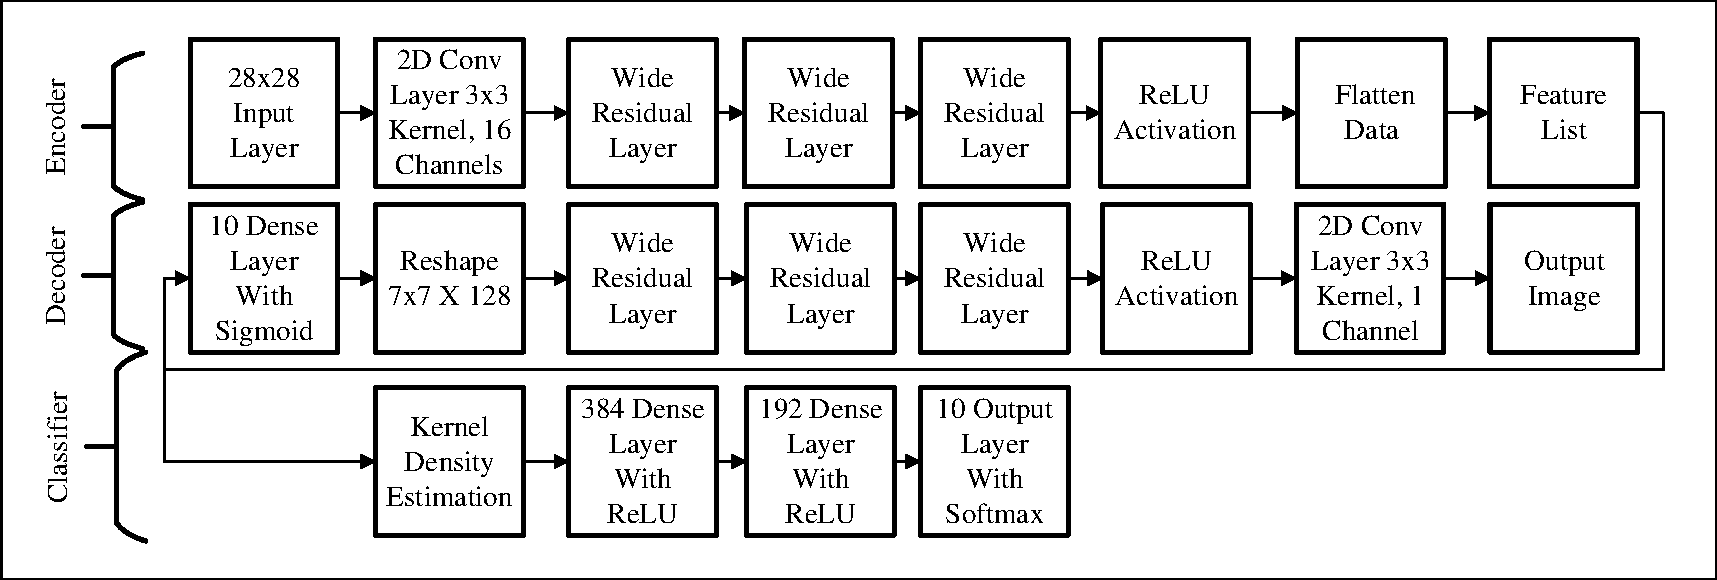
\includegraphics[width=0.7\textwidth]{images/modelarc.pdf}
    \caption{Model architecture showing a flat feature vector is obtained from the encoder, which itself takes in a $28\times28$ image. This flat vector is then passed to a decoder and a kernel density estimator, which then reconstructs and makes a softmax prediction of the UCC label respectively.}
    \label{fig:final}
\end{figure}

% The weakly supervised clustering framework consists of an end-to-end trained deep convolutional autoencoder and a classifier. Figure \ref{fig:final} shows the architecture schematic of this framework. The auto-encoder consists of $28\times28$ input layer which is passed through a 2D convolutional layer with a $3\times3$ kernel. These are then passed through a series of wide residual layers, following the architecture created by \cite{zagoruyko2016wide}, before applying a ReLU non-linearity and obtaining a flat vector consisting of encoded features extracted from the original image. A kernel density estimator is then able to infer the underlying distribution characteristics and the result of this estimation is passed to a multi-layer perceptron (MLP) with 2 hidden layers - the first consisting of 384 hidden units and the second consisting of 192 hidden units, both with ReLU activation. These produce an output with softmax over classes, representing the ten different MNIST digits. We simultaneously minimise the decoder loss so that the flat feature vectors produced at the bottleneck is densely packed with relevant information required for accurate classification. The decoder ultimately produces a reconstruction of the original image, but this is unused as its only used for the purposes of minimising loss. The model minimises a weighted sum of classification and auto-encoder losses with the weight being a hyper-parameter.

The weakly supervised clustering framework consists of an end-to-end trained deep convolutional autoencoder and a classifier. Figure \ref{fig:final} shows the architecture schematic of this framework, which can roughly be considered in three parts: the encoder, the decoder and the classifier. The encoder exists to extract features from the input images, and consists of several convolutional layers and wide residual layers, described by \cite{zagoruyko2016wide}. The extracted features are modelled by probability distributions in the Kernel Density Estimation (KDE) layer. These distributions are then fed to an MLP classifier to estimate the number of unique classes in the data. We simultaneously minimise the decoder and classifier loss so that the extracted features are specifically useful for accurate classification. The decoder ultimately produces a reconstruction of the original image, but this is unused as its only used for the purposes of minimising loss. The model minimises a weighted sum of classification and auto-encoder losses with the weight being a hyper-parameter.

% We ask the reader to note we broadly keep in line with the notation used by \cite{Oner2019}. The ucc model consists of three main modules: $\theta_{feature}$, which extracts features from each input image and produces a feature distribution; $\theta_{drn}$ which predicts ucc label; finally, $\theta_{decoder}$ uses the first module to form an auto-encoder used to improve the feature extraction process.

% The input dataset with instances $\mathcal{X} = \{x_1, x_2, \cdots, x_n\}_{i=0}^{n}$ belong to an unknown class. Through assumption of total number of unknown classes, $K$, instances are labelled $\mathcal{L}(x_i) = l_i \in \{1, 2, \cdots, K\}$ where at least one instance in the dataset belongs to one of $K$ classes. The model then predicts a label $\hat{l}_i \rightarrow \mathcal{L}(x_i) = l_i$. This is facilitated by the multiple instance learning problem where data consists of (bag, ucc) or $(\sigma,\eta_{\sigma})$ pairs and the model has to learn a concept which allows the correct prediction of $\hat{l}_i$ from the bag. The ucc $\eta_{\sigma}$ is the total number of unique classes that exist in the bag $\sigma_{\zeta}$. 

% The feature extractor module extracts features from all the instances in the bag $\theta_{feature}(x_i) = \{ f^1, f^2, \cdots, f^J \}_{i=0}^{J}$ where all feature matrices $f^i$ are accumulated for each $x_i$ to feed into the second module $\theta_{drn}$ for performing kernel density estimation (KDE) upon which distribution regression is performed to predict ucc label as a softmax vector $(\tilde{\eta^1_\sigma}, \tilde{\eta^2_\sigma}, \cdots, \tilde{\eta^K_\sigma})$. The loss function used is given in equation \ref{eqn:loss}. The distribution regression loss is minimised using cross-entropy and the auto-encoder loss minimised with mean squared error criterion; both losses are minimised concurrently in this model. 

%% justify different components like autoenc and kde

% \begin{equation}
% \alpha\left[\sum_{k=1}^{K} \eta_{\sigma}^{k} \log \tilde{\eta}_{\sigma}^{k}\right]+(1-\alpha)\left[\frac{1}{\left|\sigma\right|} \sum_{i=1}^{\left|\sigma\right|}\left(x_{i}-\tilde{x}_{i}\right)^{2}\right]
% \label{eqn:loss}
% \end{equation}

% where the hyperparameter $\alpha$ $\in [0,1]$. As we can note from the loss function in \ref{eqn:loss}, the model is trained end-to-end, with the features extracted from the auto-encoder used to automatically perform classification with a multi-layer perceptron (MLP). This attribute of unsupervised classification lends this model to be a part of weakly supervised clustering framework. 

\subsection{Training the Model} % need to mention adam optimiser
Under the weakly supervised framework, we train the UCC model to predict the number of unique classes in batches of MNIST data. Our model was trained locally using TensorFlow with Python 3.6 using a NVIDIA RTX 2070 GPU. \cite{Oner2019} train their model for 128,000 epochs, which requires $\sim12$ hours of continuous training. When compared to other simple models, this training time is orders of magnitude larger. The UCC model also demands a large amount of memory. During experimentation, we found our system undergoing excessive thrashing, as the model consumed in excess of 60GB of memory. 

\begin{figure}[htbp]
    \centering
    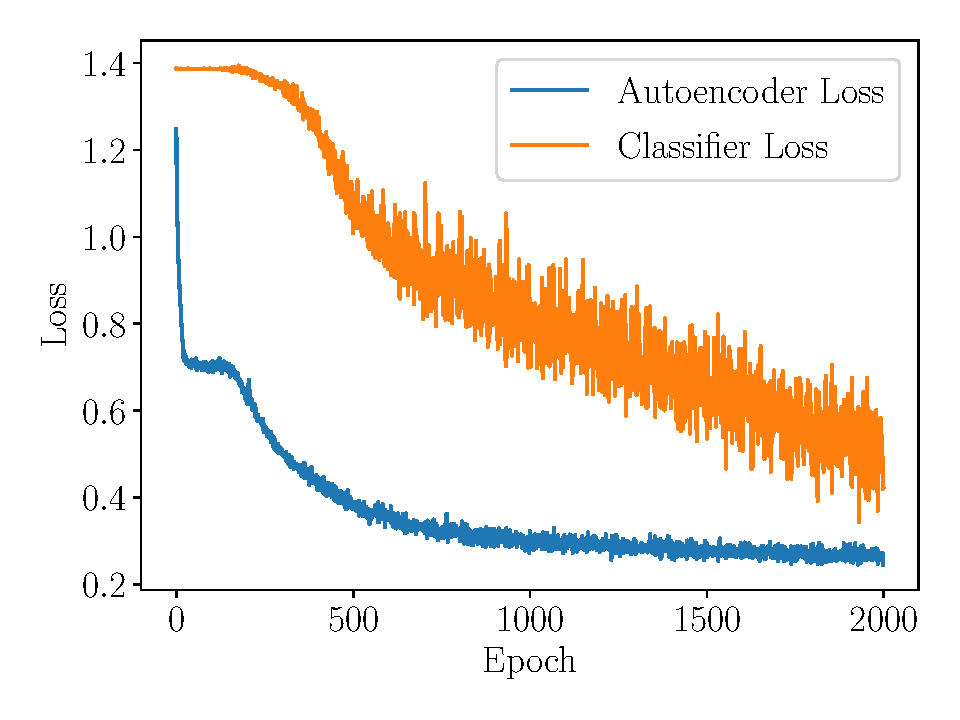
\includegraphics[scale=0.4]{images/loss_plot.pdf}
    \caption{Training loss for UCC model monotonically decreasing. The auto-encoder (blue) converges quicker than the classifier (orange).}
    \label{fig:ucc_loss}
\end{figure}

Figure \ref{fig:ucc_loss} shows the training with the described loss criterion where we find both plots are noisy. This is usually caused by a high learning rate causing instability or by a large batch size causing class imbalance as new data is seen. We experimented with both of these hyper-parameters, however this effect still persisted.

\section{Applying the Model to MNIST} %[SP]

\subsection{Autoencoder Model} %[SP]
As explained in Section \ref{sec:architecture}, the total loss of the model is dependent on the weighted sum of losses of the classifier and the autoencoder. This is intuitive, since the autoencoder needs to be able to extract ``useful'' features that the classifier can use to label the data. In this investigation, the autoencoder was trained to reduce the $28\times28$ MNIST images into a flattened list of 10 ``features'', the encoded data.

\begin{figure}[htbp]
    \centering
    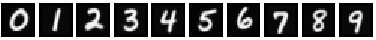
\includegraphics[scale=1]{images/digits.pdf}
    \caption{Reconstructed digits from autoencoder, which look very similar to the input images.}
    \label{fig:digits}
\end{figure}

The reconstructed digits from the MNIST data are presented in Figure \ref{fig:digits}. We immediately observe that the digits are very similar to the original MNIST data, implying that the small loss we observed in Figure \ref{fig:ucc_loss} for the autoencoder model, has led to its ability to properly encode and decode the data.

The encoded data, i.e. the feature list, could be directly fed into an MLP model for classification. However, investigations found that this produced poor results in classification, likely as a result of the small feature list. A solution is to apply certain transformations to the feature list, to obtain better classification scores. This motivates the use of KDE.

\subsection{Kernel Density Estimation Layer} %[SP]

The KDE Layer is used to construct a probability distribution of the features extracted by the autoencoder model. In this investigation, a Gaussian kernel was used, since no prior knowledge of the extracted features was known. As such, we argue that through central limit theorem, the output of a sufficiently complex encoder model can be weighted using a Gaussian kernel. 

%% Figure for distribution of features
\begin{figure}[H]
    \centering
    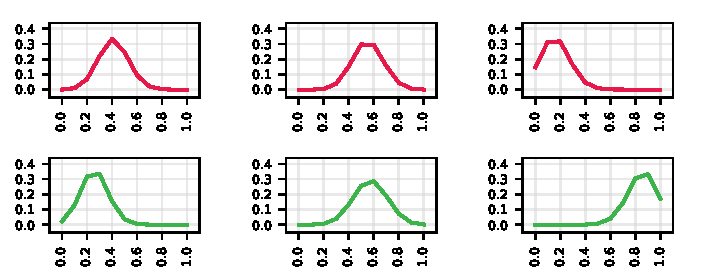
\includegraphics[scale=0.7]{images/distributions-crop.pdf}
    \caption{Distributions created by KDE layer using features from Encoder. Red shows three features distributed in class 1, and green shows three features distributed in class 2.}
    \label{fig:kde_dens}
\end{figure}

We can construct a plot of the distribution of different extracted features for different classes. This is presented in Figure \ref{fig:kde_dens}, which shows the way that features $1$, $2$ and $3$ are distributed on classes $1$ (red) and $2$ (green). We immediately observe that there are clear differences in the distributions of features for different classes. This intuitively informs us that the KDE layer can create distributions that can be easily separated into classes, resulting in higher performance of the classsifier when the KDE layer is used.

We might consider whether during inference, we can forego the MLP classifier in favour of directly clustering the distributions using an unsupervised algorithm such as K-Means. One such model is also investigated in this paper.

\subsection{Training and Inference on MNIST} %[SP]
% As mentioned, we restrict our re-implementation to working with MNIST dataset as baseline. Reproducing the results of the original paper was challenging as \cite{Oner2019} do not provide any details of the specific architectural definition of their used model. The number of epochs the original model was trained for was also very long (128000), and training our re-implemented model took $\sim12$ hours, despite being trained with a Graphical Processing unit (GPU).

The MNIST images are randomly grouped into batches of 32. We refer to these batches as ``bags''. Initially, in the training stage, the model is trained for 128000 epochs to estimate the number of unique classes in the bag. The training set is 50000 images, while the validation step is 10000 images. Early stopping is implemented, but was found to be unnecessary as overfitting on this dataset did not occur. It is possible to not have a separate training and test set, and allow the model to train on the same data upon which it will infer labels, since in the inference stage it is predicting the cluster membership and not the number of unique clusters.

Once trained, the model is used to label given instances of MNIST images into appropriate classes. We find that we achieve a clustering accuracy of \textbf{98.37$\%$}. This is close to the result found by \cite{Oner2019}. We further analyse this result and compare it with existing models in the following Section.

\subsection{Comparison with Other Models} %[SP]
We find that we can reproduce the clustering accuracy of the model created by \cite{Oner2019} with our re-implemented model. The comparisons to existing models are presented in Table \ref{tab:results}.

\begin{table}[H]
\centering
\caption{Clustering Accuracies for different models on MNIST dataset. *Models developed, trained, and tested in this investigation. Other models from other papers are shown as well.}
\vspace{0.3cm}
\label{tab:results}
\begin{tabular}{|c|c|}
\hline
\textbf{Model}                              & \textbf{Clustering Accuracy} \\ \hline
UCC Classifier*                             & 98.37\%                      \\ \hline
UCC Classifier (\cite{Oner2019})            & 98.4\%                       \\ \hline
Fully Supervised Model (\cite{Oner2019})    & 98.8\%                       \\ \hline
K-Means with Extracted Features*            & 97.73\%                      \\ \hline
K-Means with Raw Data (\cite{wang2014optimized})      & 57.2\%                       \\ \hline
IIC (\cite{ji2019invariant})                   & 98.4\%                       \\ \hline
\end{tabular}
\end{table}

We observe that with the same number of epochs and identical hyperparameters, we reproduce the original results. When we compare this model to a fully supervised model representing the upper limit of state of the art neural networks to classify MNIST data, we note that the UCC Classifier presented in this paper produces a clustering accuracy on MNIST that is very close to state of the art supervised approaches. This provides motivation for using the UCC classifier, since it can achieve high performance on weakly supervised data, comparable to a supervised model.

As suggested earlier, the classifier section of the total model (which is a simple MLP after a KDE Layer), may be superfluous during inference, as the output of the KDE distribution could be given directly to a unsupervised model to cluster. This is presented in the table, and we observe that the accuracy is very close to the total model. However, this approach still requires the use of an MLP in the training stage. As explained in Section \ref{sec:architecture}, the loss of the autoencoder is coupled to the loss of the classifier, to ensure that only features that are useful for classification are extracted by the encoder.

When we compare the results of this weakly supervised approach to a fully unsupervised K-Means algorithm applied directly to the raw data, we observe significant increases in performance, motivating the use of this weakly supervised approach. 

Finally, we compare to a state of the art unsupervised approach, presented by \cite{ji2019invariant}. We observe almost identical clustering accuracy compared to their proposed Invariant Information Clustering (IIC) approach, which does not require extensive training, or bag-level labels. This indicates that these novel unsupervised techniques might surpass this UCC Classifier approach in certain domains.

\section{Efficacy of Project}

\cite{Oner2019} present this weakly supervised clustering approach as a proof of concept. They argue that a model trained to predict the unique class count in a bag is learning patterns in the data that could be used to cluster the data into the classes. In this regard, this investigation supports their conclusions. However, we raise concerns over the practical advantage provided by such a model in a real-world setting.

We argue that the long training times ($\sim12$ hours) necessary on commercial hardware to achieve these results limits the efficacy of their presented model. When compared to models such as the IIC model presented by \cite{ji2019invariant}, the clustering accuracy is identical, but the IIC model does not require such extensive training. As such this UCC model's effectiveness is limited somewhat by the computational costs. The effectiveness of this model may vary in different domains, however.

In addition to this, the relative difficulty of reproducing the results presented by \cite{Oner2019} make the use of an identical model challenging. As they do not present specific model sizes, and fail to motivate the reasoning behind the choices made for certain architectures, it is difficult to adapt the model for other domains.

The main claim made by the original paper, however, is valid. And in many instances in which bag-level labels are available, for example in the medical field where the presence of cancerous tissue is known, even if its exact position is not, this model can prove to be superior to unsupervised techniques.

\section{Conclusions}
In this investigation we have re-implemented the UCC model presented by \cite{Oner2019} and replicated their results for the MNIST Dataset. We have also further investigated the model architecture, including by testing the model without certain components (eg. KDE layer), and provided justification for the choice of certain parts of the model. Finally, we have compared the reproduced results with existing unsupervised and supervised techniques and compared its effectiveness when factors such as the training time and model construction difficulty are considered. We argue that while the model may present benefits on other domains, its practical usefulness is outstripped by state of the art unsupervised techniques on the MNIST dataset.

% --- BIBLIOGRAPHY ---
\bibliography{iclr2019_conference}
\bibliographystyle{iclr2019_conference}

\end{document}
